\section{Uncertainties}

Radioactivity is a random process in the sense that it is not possible to predict when the next decay will occur. However, radioactivity has a mean rate of decay, which depends on the source atom.

In this experiment we



\begin{displaymath}
\begin{array}{cc}
 \text{distance(cm)} & \text{mean(cts)/Dt} 
   \\
3  &  449.92   \\
4  &  172.92   \\
5  &  84.92    \\
6  &  49.02    \\
7  &  32.38    \\
8  &  21.82    \\
9  &  15.63    \\
\end{array}
\end{displaymath}

\begin{figure}
  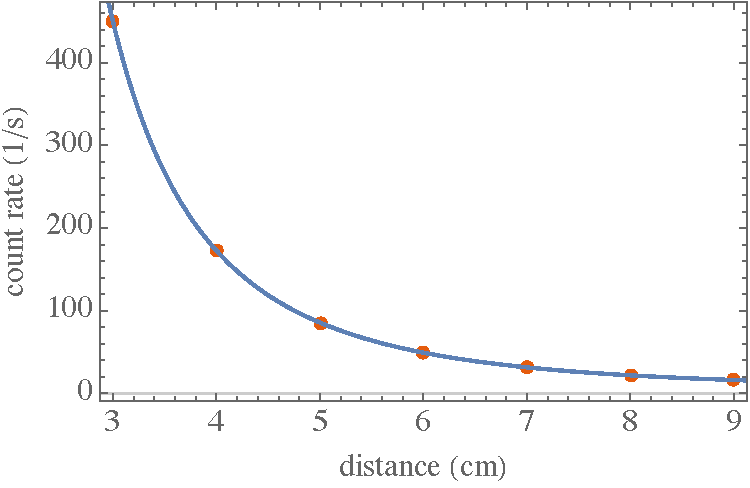
\includegraphics[width=0.5\textwidth]{Fig_Inverse_Square_Law.pdf}
\end{figure}



%\begin{problem}{3}\marginnote{\bf [15 marks]}
%Give definitions of $\sin\theta$ and $\cos\theta$ using both a right triangle and a unit circle. Draw diagrams in both cases.
%\end{problem}
